% Copyright © 2012 Martin Ueding <dev@martin-ueding.de>
%
\documentclass[11pt, ngerman, fleqn]{article}

\usepackage[a4paper, left=3cm, right=2cm, top=2cm, bottom=2cm]{geometry}
\usepackage[activate]{pdfcprot}
\usepackage[cdot, squaren]{SIunits}
\usepackage[iso]{isodate}
\usepackage[parfill]{parskip}
\usepackage[T1]{fontenc}
\usepackage[utf8]{inputenc}
\usepackage{amsmath}
\usepackage{amsthm}
\usepackage{babel}
\usepackage{color}
\usepackage{commath}
\usepackage{fancyhdr}
\usepackage{graphicx}
\usepackage{hyperref}
\usepackage{lastpage}
\usepackage{setspace}
\usepackage{tikz}

\usepackage[charter, greekuppercase=italicized]{mathdesign}

\definecolor{darkblue}{rgb}{0,0,.5}
\definecolor{darkgreen}{rgb}{0,.5,0}

\hypersetup{
	breaklinks=false,
	citecolor=darkgreen,
	colorlinks=true,
	linkcolor=black,
	menucolor=black,
	urlcolor=darkblue,
}

\setlength{\columnsep}{2cm}

\DeclareMathOperator{\arcsinh}{arsinh}
\DeclareMathOperator{\arsinh}{arsinh}
\DeclareMathOperator{\asinh}{arsinh}
\DeclareMathOperator{\card}{card}
\DeclareMathOperator{\diam}{diam}

\newcommand{\dalambert}{\mathop{{}\Box}\nolimits}
\newcommand{\divergence}[1]{\inner{\vnabla}{#1}}
\newcommand{\ee}{\mathrm e}
\newcommand{\emesswert}{\del{\messwert \pm \messwert}}
\newcommand{\ev}{\hat{\vec e}}
\newcommand{\e}[1]{\cdot 10^{#1}}
\newcommand{\fehlt}{\textcolor{red}{Hier fehlen noch Inhalte.}}
\newcommand{\half}{\frac 12}
\newcommand{\ii}{\mathrm i}
\newcommand{\inner}[2]{\left\langle #1, #2 \right\rangle}
\newcommand{\laplace}{\mathop{{}\Deltaup}\nolimits}
\newcommand{\messwert}{\textcolor{blue}{\square}}
\newcommand{\punkte}{\textcolor{white}{xxxxx}}
\newcommand{\tens}[1]{\boldsymbol{\mathsf{#1}}}
\newcommand{\vnabla}{\vec \nabla}
\renewcommand{\vec}[1]{\boldsymbol{#1}}

\newcommand{\themodul}{physik321}
\newcommand{\thegruppe}{Gruppe 8 -- Julia Volmer}
\newcommand{\theuebung}{6}

\pagestyle{fancy}

\fancyfoot[C]{\footnotesize{\thegruppe}}
\fancyfoot[L]{\footnotesize{Martin Ueding, Simon Schlepphorst}}
\fancyfoot[R]{\footnotesize{Seite \thepage\ / \pageref{LastPage}}}
\fancyhead[L]{\themodul{} -- Übung \theuebung}

\def\thesection{H \theuebung.\arabic{section}}
\def\thesubsubsection{\thesubsection\alph{section}}

\title{\themodul{} -- Übung \theuebung \\ \vspace{0.5cm} \large{\thegruppe}}

\author{
	Martin Ueding \\ \small{\href{mailto:mu@uni-bonn.de}{mu@uni-bonn.de}}
	\and
	Simon Schlepphorst \\ \small{\href{mailto:s2@uni-bonn.de}{s2@uni-bonn.de}}
}

\begin{document}

\maketitle

\begin{table}[h]
	\centering
	\begin{tabular}{l|c|c|c|c|c}
		Aufgabe & \ref 1 & \ref 2 & \ref 3 & \ref 4 & $\sum$   \\
		\hline
		Punkte & \punkte / 10 & \punkte / 10 & \punkte / 20 & \punkte / 10 & \punkte / 50
	\end{tabular}
\end{table}

%%%%%%%%%%%%%%%%%%%%%%%%%%%%%%%%%%%%%%%%%%%%%%%%%%%%%%%%%%%%%%%%%%%%%%%%%%%%%%%
%                                 Lorenzkraft                                 %
%%%%%%%%%%%%%%%%%%%%%%%%%%%%%%%%%%%%%%%%%%%%%%%%%%%%%%%%%%%%%%%%%%%%%%%%%%%%%%%

\section{Lorenzkraft}
\label 1

\subsection{qualitative Teilchenbahn und Bewegungsgleichungen}

Das Teilchen ist im konservativen $\vec E$-Feld. Dort fällt es entlang des
Feldes, wird allerdings vom $\vec B$-Feld abgelenkt und wird gegen das Feld
gelenkt. Das Teilchen kommt nur so weit, bis es die $z$-Stelle des
Anfangspunkts erreicht hat. Das ganze hatte ich in der Schule in einer Aufgabe,
dazu hatte ich ein Programm
geschrieben\footnote{\url{http://martin-ueding.de/projects/van-allen-sim-3d/}}.
Ein Bildschirmfoto des Programms ist in Abbildung \ref{fig:ebsim}.

\begin{figure}
	\centering
	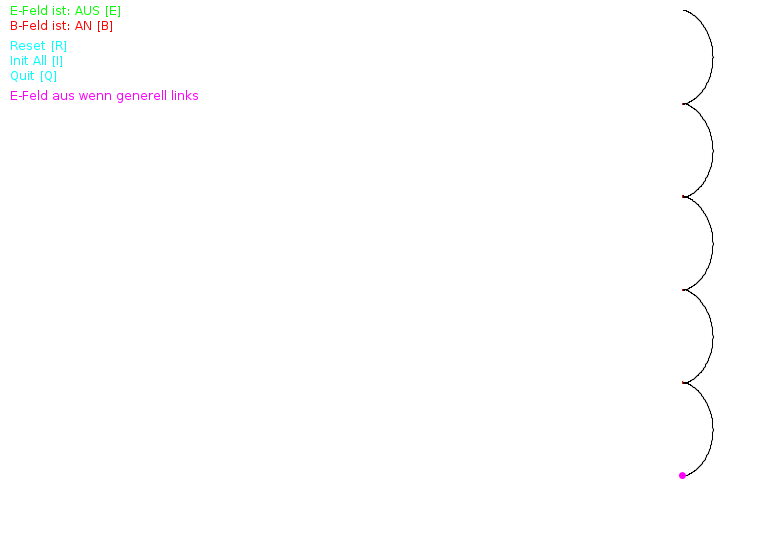
\includegraphics[width=.5\textwidth]{ebsim2.png}
	\caption{Bildschirmfoto des Programms}
	\label{fig:ebsim}
\end{figure}


Das Teilchen bewegt sich auf einer Zykloiden, im Mittel senkrecht zu $\vec E$-
und $\vec B$-Feld, also entlang der $y$-Achse.

Die Kraft auf das Teilchen ist:
\[
	\vec F = q \del{\vec E + \vec v \times \vec B}
\]

In Komponenten geschrieben:
\[
	\ddot r^i = \frac qm \del{E \delta^i{}_z + \epsilon^i{}_{jk} \dot r^j B \delta^k{}_x}
\]

Daraus ergeben sich drei gekoppelte, partielle Differentialgleichungen:
\[
	\ddot x = 0
	,\quad
	\ddot y = \frac qm \dot z B
	,\quad
	\ddot z = \frac qm \del{E - \dot y B}
\]

Für $x$ gilt aufgrund der Anfangsbedingungen: $x(t) = 0$. Die Gleichungen für
$y$ und $z$ können wir jeweils nach der Zeit ableiten und in die Andere
einsetzen. So erhalten wir zwei unabhängige Differentialgleichungen höherer
Ordnung:
\[
	\dddot y = \frac{q^2}{m^2} B E - \frac{q^2}{m^2} B^2 \dot y
	,\quad
	\dddot z = - \frac{q^2}{m^2} B^2 \dot z
\]

Diese Bewegungen sind, von additiven linearen Bewegungen abgesehen, harmonische
Schwingungen.

\subsection{Lösung der Gleichungen}

Die zu $y$ gehörige homogene Gleichung können wir durch Kosinus und Sinus
lösen:
\[
	y_h(t) = c_1 \cos\del{\omega t} + c_2 \sin\del{\omega t}
\]

Dabei haben wir schon die Ersetzung $\omega := q B / m$ vorgenommen. Als
inhomogene Lösung erraten wir:
\[
	y_p(t) = \frac EB t + c_3
\]

Somit gilt für $y$:
\[
	y(t) = c_1 \cos\del{\omega t} + c_2 \sin\del{\omega t} + \frac EB t + c_3
\]

Ähnlich gehen wir für $z$ vor und erhalten:
\[
	z(t) = c_4 \cos\del{\omega t} + c_5 \sin\del{\omega t} + c_6
\]

Die komplette Lösung für den Positionsvektor $\vec r$ ist somit:
\[
	\vec r(t) = \begin{pmatrix}
		0 \\
		c_1 \\
		c_4 \\
	\end{pmatrix} \cos\del{\omega t}
	+
	\begin{pmatrix}
		0 \\
		c_2 \\
		c_5 \\
	\end{pmatrix} \sin\del{\omega t}
	+
	\begin{pmatrix}
		0 \\
		\frac EB \\
		0 \\
	\end{pmatrix} t
	+
	\begin{pmatrix}
		0 \\
		c_3 \\
		c_6 \\
	\end{pmatrix}
\]

Nun war in der Aufgabenstellung gefordert, dass $\vec r(0) = \dot{\vec r}(0) =
\vec 0$. Die Ableitung nach der Zeit ist:
\[
	\dot{\vec r}(t) = \begin{pmatrix}
		0 \\
		- \omega c_1 \\
		- \omega c_4 \\
	\end{pmatrix} \sin\del{\omega t}
	+
	\begin{pmatrix}
		0 \\
		\omega c_2 \\
		\omega c_5 \\
	\end{pmatrix} \cos\del{\omega t}
	+
	\begin{pmatrix}
		0 \\
		\frac EB \\
		0 \\
	\end{pmatrix}
\]

Daraus erhalten wir:
\[
	c_2 = - \frac{E}{\omega B}
	,\quad
	c_5 = 0
\]

Weil wir die Gleichungen zur Lösung noch einmal abgeleitet hatten, müssen wir
noch die Bedingung $\ddot{\vec r}(0) = \frac qm E \ev_z$ erfüllen. Somit erhalten wir noch:
\[
	\dot{\vec r}(0) = \begin{pmatrix}
		0 \\
		- \omega^2 c_1 \\
		- \omega^2 c_4 \\
	\end{pmatrix}
	= \frac qm E \ev_z
\]

Dies können wir umstellen und erhalten zusammen mit $c_1 + c_3 = 0$ sowie $c_4
+ c_6 = 0$ aus $\dot{\vec r}(0) = \vec 0$:
\[
	c_1 = 0
	,\quad
	c_3 = 0
	,\quad
	c_4 = - \frac{E}{\omega B}
	, \quad
	c_6 = \frac{E}{\omega B}
\]

Alles zusammen ergibt die Bahnkurve:
\[
	\vec r(t) = - \frac{E}{\omega B} \begin{pmatrix}
		0 \\
		\sin\del{\omega t} \\
		\cos\del{\omega t} \\
	\end{pmatrix}
	+
	\begin{pmatrix}
		0 \\
		\frac EB \\
		0 \\
	\end{pmatrix} t
	+
	\begin{pmatrix}
		0 \\
		0 \\
		\frac{E}{\omega B} \\
	\end{pmatrix}
\]

Die Bahnkurve ist für $t \in \intoo{0, 15}$ in Abbildung \ref{fig:zyklo}
dargestellt. Dies stimmt mit den Überlegungen und der Simulation (Abbildung
\ref{fig:ebsim}) überein.

\begin{figure}
	\centering
	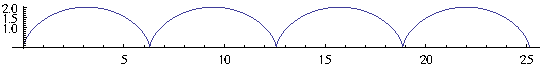
\includegraphics[width=0.7\textwidth]{1-zyklo.pdf}
	\caption{Bahnkurve $\vec r(t)$ für $t \in \intoo{0, 15}$}
	\label{fig:zyklo}
\end{figure}

%%%%%%%%%%%%%%%%%%%%%%%%%%%%%%%%%%%%%%%%%%%%%%%%%%%%%%%%%%%%%%%%%%%%%%%%%%%%%%%
%                         Kraft auf elementaren Dipol                         %
%%%%%%%%%%%%%%%%%%%%%%%%%%%%%%%%%%%%%%%%%%%%%%%%%%%%%%%%%%%%%%%%%%%%%%%%%%%%%%%

\section{Kraft auf elementaren Dipol}
\label 2

Zuerst bestimmen wir das magnetische Moment der Leiterschleife. Die Definition lautet:
\[
	\vec m = \half \int \dif^3 x \del{\vec r \times \vec j\del{\vec r}}
\]

Da nur auf der Leiterschleife Strom fließt, können wir das Integral auf die
vier Kanten zerlegen. Dabei gehen wir davon aus, dass der Strom gemäß der
rechten Hand um die $x$-Achse fließt. Wir könnten die Stromdichte aus einer
Summe von $\delta$-Distributionen zusammensetzen, diesen Schritt überspringen
wir. Das magnetische Moment ist also über alle vier Kanten zusammen:
\begin{align*}
	\vec m
	&= \half \int \dif^3 r \del{\vec r \times \vec j\del{\vec r}} \\
	&= \half I \del{
	\int_0^\varepsilon \dif y
	\begin{pmatrix}
		0 \\ y \\ 0
	\end{pmatrix}
	\times
	\ev_y
	+
	\int_0^\varepsilon \dif z
	\begin{pmatrix}
		0 \\ \varepsilon \\ z
	\end{pmatrix}
	\times
	\ev_z
	-
	\int_0^\varepsilon \dif y
	\begin{pmatrix}
		0 \\ y \\ \varepsilon
	\end{pmatrix}
	\times
	\ev_y
	-
	\int_0^\varepsilon \dif z
	\begin{pmatrix}
		0 \\ 0 \\ z
	\end{pmatrix}
	\times
	\ev_z
} \\
	&= \half I \del{
	\int_0^\varepsilon \dif y
	\begin{pmatrix}
		0 \\ 0 \\ \varepsilon
	\end{pmatrix}
	+
	\int_0^\varepsilon \dif z
	\begin{pmatrix}
		0 \\ 0 \\ \varepsilon
	\end{pmatrix}
} \\
&= I \varepsilon^2 \ev_x
\end{align*}

Dies stimmt mit dem in der Aufgabenstellung gegebenen Betrag $m = I \varepsilon^2$
überein.

Nun betrachten wir die Kraft auf das Leiterschlaufe:
\begin{align*}
	\vec F
	&= \oint \dif l \del{\vec I \times \vec B} \\
	\intertext{Die magnetische Flussdichte können wir mit der gegebenen Näherung annähern. Dabei schreiben wir $B_{0,i} := B_i(0, 0, 0)$, und $B_i := \eval[2]{\pd Bi}_{\vec r = \vec 0}$.}
	&=
	\int_0^\varepsilon \dif y
	\begin{pmatrix}
		0 \\ I \\ 0
	\end{pmatrix}
	\times
	\begin{pmatrix}
		B_{0,x} \\ B_{0,y} + B_y y \\ B_{0,z}
	\end{pmatrix}
	+
	\int_0^\varepsilon \dif z
	\begin{pmatrix}
		0 \\ 0 \\ I
	\end{pmatrix}
	\times
	\begin{pmatrix}
		B_{0,x} \\ B_{0,y} + B_y \varepsilon \\ B_{0,z} + B_z z
	\end{pmatrix} \\
	&\quad
	-
	\int_0^\varepsilon \dif z
	\begin{pmatrix}
		0 \\ I \\ 0
	\end{pmatrix}
	\times
	\begin{pmatrix}
		B_{0,x} \\ B_{0,y} + B_y y \\ B_{0,z} + B_z \varepsilon
	\end{pmatrix}
	-
	\int_0^\varepsilon \dif y
	\begin{pmatrix}
		0 \\ 0 \\ I
	\end{pmatrix}
	\times
	\begin{pmatrix}
		B_{0,x} \\ B_{0,y} \\ B_{0,z} + B_z z
	\end{pmatrix} \\
	&=
	I \del{
	\int_0^\varepsilon \dif y
	\begin{pmatrix}
		B_{0,z} \\ 0 \\ - B_{0,x}
	\end{pmatrix}
	-
	\begin{pmatrix}
		B_{0,z} + B_{0,z} \varepsilon \\ 0 \\ - B_{0,x}
	\end{pmatrix}
	}
	+
	I \del{
	\int_0^\varepsilon \dif y
	\begin{pmatrix}
		- B_{0,y} - B_y \varepsilon \\ B_{0,x} \\ 0
	\end{pmatrix}
	-
	\begin{pmatrix}
		- B_{0,y} \\ B_{0,x} \\ 0
	\end{pmatrix}
	} \\
	&=
	I \varepsilon \del{
	\begin{pmatrix}
		B_{0,z} \\ 0 \\ - B_{0,x}
	\end{pmatrix}
	-
	\begin{pmatrix}
		B_{0,z} + B_{0,z} \varepsilon \\ 0 \\ - B_{0,x}
	\end{pmatrix}
	+
	\int_0^\varepsilon \dif y
	\begin{pmatrix}
		- B_{0,y} - B_y \varepsilon \\ B_{0,x} \\ 0
	\end{pmatrix}
	-
	\begin{pmatrix}
		- B_{0,y} \\ B_{0,x} \\ 0
	\end{pmatrix}
	} \\
	\intertext{Der konstante Teil des Magnetfeldes hat nette keine Kraft auf die Leiterschleife, da der Strom in den gegenüberliegenden Seiten gerade entgegengesetzt fließt.}
	&= I \varepsilon^2 \del{-B_z - B_y} \ev_x \\
	&= - I \varepsilon^2 \divergence{\vec B} \ev_x \\
	\intertext{An dieser Stelle können wir Gradienten von $B_x$ addieren, weil es durch die Näherung konstant ist und somit 0 addiert wird.}
	&= - I \varepsilon^2 \del{\divergence{\vec B} \ev_x - \vnabla B_x} \\
	\intertext{Ab hier betrachten wir noch noch die $i$-Komponente der Kraft.}
	F^i
	&= - I \varepsilon^2 \del{\delta^i{}_x \partial_b B^b - \partial^i B_x} \\
	\intertext{Hier führen wir noch mehr Indizes ein.}
	&= - I \varepsilon^2 \del{\delta_k{}^b \delta^i{}_x \partial_b B^k - \delta_{kx} \delta^{ib} \partial_b B^k} \\
	&= I \varepsilon^2 \del{\delta_{kx} \delta^{ib} - \delta_k{}^b \delta^i{}_x} \partial_b B^k \\
	\intertext{Diese vier $\delta$ können wir nun als zwei, mit einem Index kontrahierten, $\tens \epsilon$-Tensoren zusammenfassen.}
	&= \epsilon_{jk}{}^i \epsilon^j{}_x{}^b I \varepsilon^2 \partial_b B^k \\
	\intertext{Wir führen einen weitern Index $a$ ein.}
	&= \epsilon_{jk}{}^i \epsilon^j{}_a{}^b I \varepsilon^2 \delta_x{}^a \partial_b B^k \\
	\intertext{Jetzt können wir das vorher bestimmte magnetische Moment $\vec m$ einsetzen. Dabei müssen wir natürlich nur die entsprechende, $x$-Komponente einsetzen.}
	&= \epsilon_{jk}{}^i \epsilon^j{}_a{}^b m^a \partial_b B^k \\
	\intertext{Nun permutieren wir die Indizes am ersten $\tens \epsilon$-Tensor.}
	&= \epsilon^i{}_{jk} \epsilon^j{}_a{}^b m^a \partial_b B^k \\
	\intertext{Zur Übersicht können wir noch den mittleren Term als eigenen Vektor schreiben.}
	&= \epsilon^i{}_{jk} \del{\epsilon_{na}{}^b m^a \partial_b \ev^n}^j B^k \\
	\intertext{Dies ist nun ein doppeltes Kreuzprodukt.}
	&= \del{ \vec m \times \vnabla} \times B
\end{align*}

Und das ist genau die gesuchte Relation.

%%%%%%%%%%%%%%%%%%%%%%%%%%%%%%%%%%%%%%%%%%%%%%%%%%%%%%%%%%%%%%%%%%%%%%%%%%%%%%%
%                              Helmholtz-Spulen                               %
%%%%%%%%%%%%%%%%%%%%%%%%%%%%%%%%%%%%%%%%%%%%%%%%%%%%%%%%%%%%%%%%%%%%%%%%%%%%%%%

\section{Helmholtz-Spulen}
\label 3

\subsection{Herleitung des Potentials}

\fehlt

\subsection{homogenes Feld}

Es soll gezeigt werden, dass das Feld bei $R = 2a$ homogen ist. Dazu bilde ich
$\vec B = \vnabla \times \vec A$ in Zylinderkoordinaten. Es gilt $\vec A = A_y
\phi$. Die Rotation ist:
\[
	\vec B = \del{\frac 1\rho \dpd{A_z}\phi - \dpd{A_\phi}z} \ev_\rho
	+ \del{\dpd{A_\rho}z - \dpd{A_z}\rho} \ev_\phi
	+ \frac 1\rho \del{\dpd{\del{\rho A_\phi}}\rho - \dpd{A_\rho}\phi} \ev_z
\]

Dabei sind nur zwei Terme nicht null. Diese sind:
\[
	\dpd{A_\phi}z = \frac{\mu_0 I \rho R^2}{2 \del{R^2 + a^2}^{3/2}} \del{- \frac{3z}{R^2 + a^2} + \frac{15 a^2 z}{\del{R^2+a^2}^2}}
\]
\[
	\frac 1\rho \dpd{\del{\rho A_\phi}}\rho
	=
	\frac{\mu_0 I \rho R^2}{\del{R^2+a^2}^{3/2}} \del{1- \frac 32 \frac{z^2 + \rho^2}{R^2 + a^2} + \frac{15}8 \frac{R^2 \rho^2 + 4 a^2 z^2}{\del{R^2 + a^2}^2} - \frac{3\rho^2}{R^2+a^2} + \frac{15}4 \frac{R^2 \rho^2}{\del{R^2+a^2}^2}}
\]

Wir kombinieren die beiden Komponenten und setzen $R := 2a$ ein. Damit fallen
alle Terme in den Klammern, bis auf die $1$ im zweiten Term weg, so dass das
$\vec B$-Feld ist:
\[
	\vec B = \frac{4 \mu_0 I a^2}{\del{5a^2}^{3/2}} \ev_z
\]

Dies ist in der Tat homogen.

%%%%%%%%%%%%%%%%%%%%%%%%%%%%%%%%%%%%%%%%%%%%%%%%%%%%%%%%%%%%%%%%%%%%%%%%%%%%%%%
%               Eigenschaften ebener elektromagnetischer Wellen               %
%%%%%%%%%%%%%%%%%%%%%%%%%%%%%%%%%%%%%%%%%%%%%%%%%%%%%%%%%%%%%%%%%%%%%%%%%%%%%%%

\section{Eigenschaften ebener elektromagnetischer Wellen}
\label 4

\fehlt

%\bibliography{../../zentrale_BibTeX/Central}
%\bibliographystyle{plain}

\end{document}

% vim: spell spelllang=de
